\documentclass{beamer}

\usepackage{gensymb}
\usepackage[utf8]{inputenc}
\DeclareUnicodeCharacter{00A0}{ }%Permet d'éviter certains conflits de caractères invisibles
\usepackage{amssymb}            % Principaux symboles
%\usepackage{fontspec}
%\usepackage{xunicode}
%\usepackage{xltxtra}
\usepackage[frenchb]{babel}
%\defaultfontfeatures{Scale=MatchLowercase}
%\setmainfont[Mapping=tex-text,Ligatures={Common, Historical}]{Linux Libertine O}
%\setsansfont[Mapping=tex-text]{Linux Biolinum O}
%\setmonofont[Scale=0.75]{DejaVu Sans Mono}

%% Packages pour le texte
%\usepackage[misc,geometry]{ifsym}	% Police numéros battons
\usepackage{pifont}		% Police \ding
\usepackage{eurosym}		% Symbole de l'euro
\usepackage{soul}		% Souligner
\usepackage{enumerate}		% Listes
\usepackage{verbatim}		% Codes source
\usepackage{moreverb}		%	et listings
\usepackage{textcomp}
\usepackage{multicol}

%% Packages pour les tableaux
\usepackage{array}		% Outils supplémentaires
\usepackage{multirow}		% Colonnes multiples
\usepackage{tabularx}		% Largeur totale donnée
\usepackage{longtable}		% Sur plusieurs pages

%% Les packages pour les dessins
\usepackage{graphicx}		% Insertion de figures
%\usepackage{picins}		% Dans un paragraphe
\usepackage{epic}		% Capacités graphiques
\usepackage{eepic}		% 	étendues
\usepackage{afterpage}		% Voir page 69
\usepackage{rotating}		% Tourner du texte
\usepackage{caption}		% Légendes
% \addto\captionsfrench{\def\figurename{}}

%% Packages pour les maths
\usepackage{amsmath}		% Commandes essentielles
\usepackage{amssymb}		% Principaux symboles
\usepackage{mathrsfs}		% Police calligraphique
\usepackage{theorem}		% Théorèmes
%\usepackage{tikz}		% Courbes
\usepackage{esvect}            % Vecteurs
%\usetikzlibrary{shapes,arrows,shadows}
\usepackage{pgf}
%\usetikzlibrary{arrows}
% Packages pour la physique
%\usepackage{sistyle}		% Unités
\usepackage[version=3]{mhchem}	% Formules chimiques
\usepackage{etex}
%\usepackage{m-pictex,m-ch-en}

%\usepackage{media9}
\usepackage{multimedia}		% Vidéos dans la présentation
%\usepackage{movie15}

%Ajout d'images de fond:
\usepackage{eso-pic}
\usepackage{wallpaper}

\usepackage{ccicons}		% Licence creativecommons

%\SIdecimalsign{,}


\AtBeginSection[]
{
  \begin{frame}
    \frametitle{Sommaire}
    \begin{multicols}{2}
      {\small
				\setcounter{tocdepth}{2}
        \tableofcontents[currentsection, hideothersubsections]}
    \end{multicols}
  \end{frame}
}

\usetheme{Warsaw}

\usepackage{listings}
\usepackage[babel=true]{csquotes}
\lstset{language=Python, tabsize=2, breaklines=true, showstringspaces=false}

\useoutertheme{infolines}
\setbeamersize{text margin left=1cm,text margin right=1cm}

\title{Rapport de projet de SI}
\subtitle{Tropodrone}
\author{Gueydan Noé, Manceau Thibaut, Gros Alexis, Porteries Tristan}

\begin{document}

\begin{frame}
  \titlepage
\end{frame}

\begin{frame}
    \frametitle{Sommaire}
    \begin{multicols}{2}
      {
		\setcounter{tocdepth}{1}
        \tableofcontents
      }
    \end{multicols}
\end{frame}

\section{Courte présentation}

\subsection{But du projet}
\begin{frame}{But du projet}
 Créer une structure composée de ballons contenant un gaz plus léger que l’air qui soutient une partie ou la totalité du poids d'un drone.
\end{frame}


\subsection{Objectifs}
\begin{frame}{Objectifs}
 Augmenter l’autonomie, la sécurité et les possibilités d’un drone de petite taille
\end{frame}


\subsection{Contraintes imposées au projet}
\begin{frame}{Contraintes imposées au projet}
  \begin{itemize}
    \item Être simple d’utilisation, garder la manœuvrabilité du drone au possible, voler le plus longtemps possible.
    \item Consommer le moins d’énergie possible, ne pas présenter de danger pour le public et économiser le gaz et les matériaux de fabrication.
    \item Le modèle du drone imposé
    \item Rayon d’action de minimum 15 mètres
    \item Ballon de type dirigeable
  \end{itemize}
\end{frame}

\subsection{Contraintes légales supplémentaires}
\begin{frame}{Contraintes légales supplémentaires}
  \begin{itemize}
    \item 1: Le drone \\
	    Catégorie A : limitations non contraignantes
    \item 2: Le ballon \\
	    Catégorie « Léger » \\
	    La ficelle supportant la charge doit casser au dessus de 23 kg
 \end{itemize}
\end{frame}

\section{Calculs d'élévation}

\subsection{Poussé d'archimède}

\begin{frame}{Définition}
  \enquote{Tout corps plongé dans un fluide au repos, entièrement mouillé par celui-ci ou traversant sa surface libre, subit une force verticale, dirigée de bas en haut et opposée au poids du volume de fluide déplacé ; cette force est appelée poussée d'Archimède.}
  \bigbreak
  \begin{center}
    \boxed{\vv{Pa} = -M_F \times \vv{g}}
  \end{center}
  \begin{itemize}
    \item $\vv{Pa}$~: la poussé d'archimède~;
    \item $M_F$~: la masse du fluide contenue dans le volume déplacé~;
    \item $\vv{g}$~: la valeur du champ de pesanteur.
  \end{itemize}
\end{frame}

\begin{frame}{Application aux gaz}
  Deux forces appliquées sur le ballon~: \\
  \begin{center}
    $\displaystyle{\vv{F_{ballon}} = \vv{P_{ballon}} + \vv{Pa_{ballon}}}$ \\
  \end{center}
  Si $P_{ballon} < Pa_{ballon}$ la force d'élévation est~:
  \begin{center}
    $\displaystyle{F_{ballon} = Pa_{ballon} - P_{ballon}}$ \\
  \end{center}
  Remarque~:\\
  \begin{center}
    $F_{ballon} < Pa_{ballon}$
  \end{center}
\end{frame}

\subsection{Dilatation des gaz}

\begin{frame}{Loi de Charles}
  \begin{center}
    \boxed{\displaystyle{\frac{V_1}{T_1} = \frac{V_2}{T_2} = f(P, n)}} \\
    $\displaystyle{V_3 = f(P, n) \times T_3}$
  \end{center}
  Avec~:
  \begin{itemize}
    \item $V_q$~: volume du gaz en $m^3$ à la température $T_q$ en K~;
    \item $P$~: pression du gaz en Pa~;
    \item $n$~: quantité de matière en mol~;
    \item $f(P, n)$~: rapport constant entre volume et température.
  \end{itemize}
\end{frame}

\begin{frame}{Application à l'hélium}
  Volume molaire de l'hélium~: $22.414\times 10^{-3} m^3.mol^{-1}$ à $273.25K$.
  \begin{center}
    $\displaystyle{f(P, n) = \frac{22.414\times 10^{-3}}{273.25} = 8.2\times 10^{-5} m^3.mol^{-1}.K^{-1}}$
  \end{center}
  Pour $T_{200} = 200 \degree C = 473.25 K$~:
  \begin{center}
    $\displaystyle{V_{T_{200}} = 8.2\times 10^{-5} * 473.25 = 38.811 \times 10^{-3}} m^3.mol^{-1}$
  \end{center}
  Augmentation du volume de $1.59$.
\end{frame}

\begin{frame}{Application à l'hydrogène}
  Volume molaire de l'hélium~: $22.414\times 10^{-3} m^3.mol^{-1}$ à $273.25K$.
  \begin{center}
    $\displaystyle{f(P, n) = \frac{22.414\times 10^{-3}}{273.25} = 8.2\times 10^{-5} m^3.mol^{-1}.K^{-1}}$
  \end{center}
  Pour $T_{200} = 200 \degree C = 473.25 K$~:
  \begin{center}
    $\displaystyle{V_{T_{200}} = 8.2\times 10^{-5} * 473.25 = 38.811 \times 10^{-3}} m^3.mol^{-1}$
  \end{center}
  Augmentation du volume de $1.59$.
\end{frame}

\begin{frame}{Résultat de la poussé d'archimède}
  \begin{center}
    $\displaystyle{F_{T_0} = Pa_{air} - P_{helium} = 10.90 N}$
    \bigbreak
    $\displaystyle{F_{T_{200}} = Pa_{air} - \frac{P_{helium}}{1.59} = 11.57 N}$ \\
  \end{center}
  Les resultats sont négligables. $F < Pa_{air}$
\end{frame}

\section{Structure}

\subsection{Piloter le drone}

\begin{frame}
  La structure~: piloter le drone.
  Les contraintes~:
  \begin{itemize}
    \item mobilité~;
    \item rigidité~;
    \item légerté~;
    \item légalité.
  \end{itemize}
\end{frame}

\begin{frame}{Les solutions techniques}
  Légerté et rigidité~: fibres de carbonne Répartition des matériaux et expériences.
  \begin{center}
    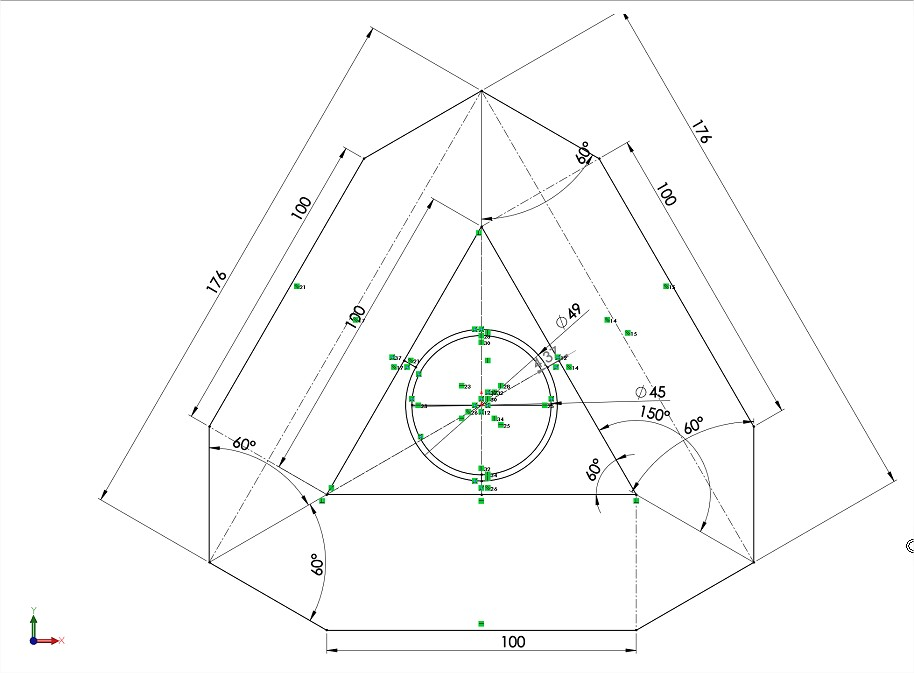
\includegraphics[width=8cm]{../Images/plan_structure.jpg}
  \end{center}
\end{frame}

\begin{frame}{Mobilité}
  Forme triangulaire des ballons, centre de gravité, le même que celui du drone, quantité d'hélium. \\
  Structure gyroscopique.
  \begin{center}
    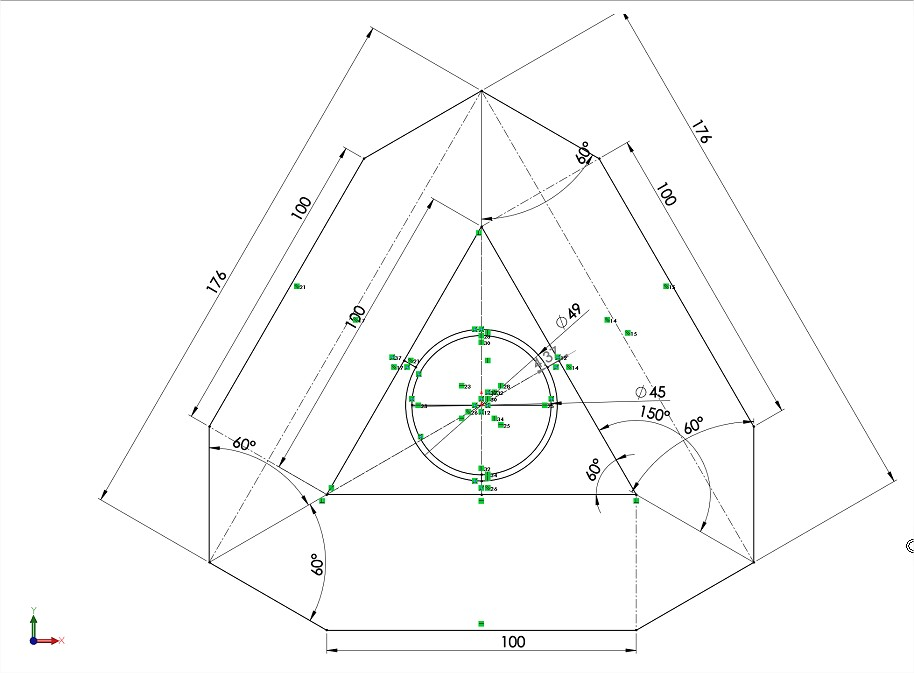
\includegraphics[width=7cm]{../Images/plan_structure.jpg}
  \end{center}
\end{frame}

\subsection{Attaches et modélisation}

\begin{frame}
  \begin{center}
    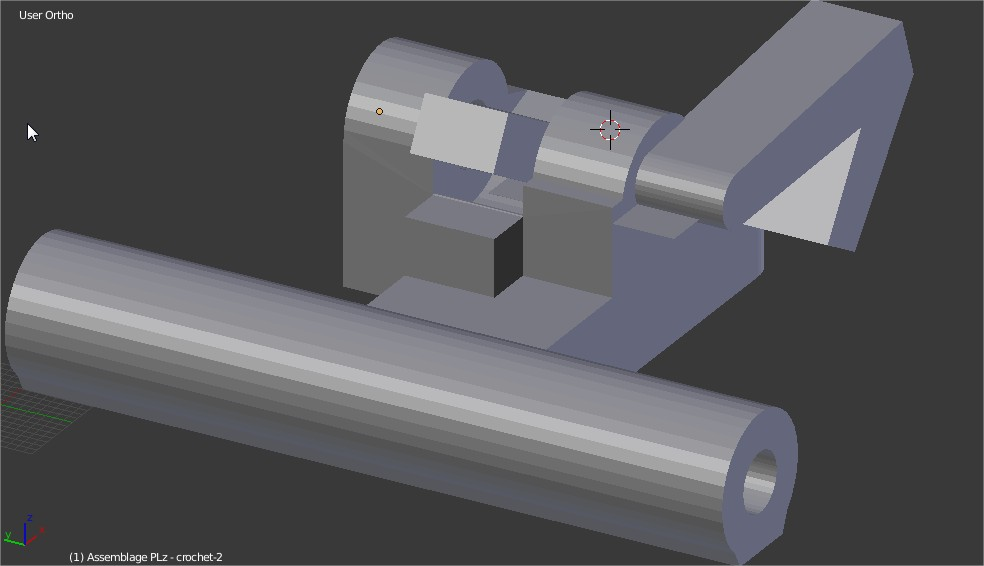
\includegraphics[width=10cm]{../Images/fixation.jpg}
  \end{center}
  \captionof{figure}{Fixation triangle-premier cercle.}
\end{frame}

\section{Ballon}

\subsection{Contenance}

\subsection{Forme}

\begin{frame}
  Les ballon sont formés d'un parallèlépipède avec deux pyramides d'angle $60\degree$. \\
  \begin{center}
    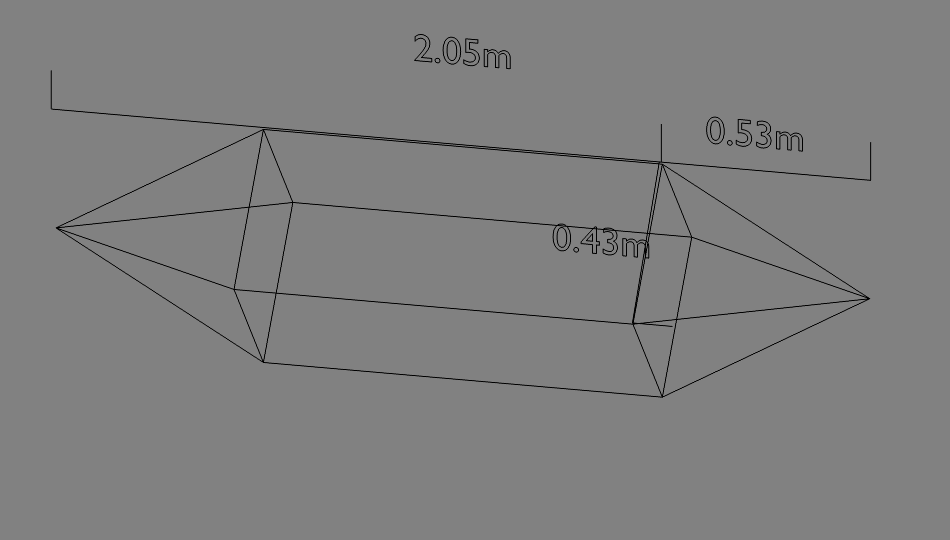
\includegraphics[width=10cm]{../Images/ballon.png}
  \end{center}
\end{frame}

\begin{frame}{Calcul des dimensions}
  Volume ballon~:
  \begin{center}
    \boxed{\displaystyle{V = 2(b^2 (b \sin \frac{\pi}{3} \times \frac{1}{3})) + b^2}} \\
    $\displaystyle{V = b^3 \frac{\sqrt{3}}{3} + b^2}$ \\
    $\displaystyle{b^3 \frac{\sqrt{3}}{3} + b^2 - 0.25 = 0}$
  \end{center}
  Polynome du troisième degrée, résolution par bissection ou dichotomie.
\end{frame}

\begin{frame}[fragile]{Résolution par bissection}
  \begin{lstlisting}[frame=single]
etape = 1
largeur = 1
vol = volume(largeur)
cible = 0.25
epsilon = 1e-4
while abs(vol - cible) > epsilon:
	if vol < cible:
		largeur += etape
	else:
		largeur -= etape
	etape /= 2
	vol = volume(largeur)

print("volume = %f, diametre = %f" % (vol, largeur))
  \end{lstlisting}
\end{frame}

\subsection{Enveloppe}

\begin{frame}
  \begin{multicols}{2}
    \begin{itemize}
      \item Latex~:
      \begin{itemize}
        \item facile à trouver dans le commerce,
        \item seulement en forme sphèrique,
        \item peu étanche~;
      \end{itemize}
      \item Chloroprène~:
      \begin{itemize}
        \item introuvable dans le commerce~;
      \end{itemize}
      \item Butyle~:
      \begin{itemize}
        \item introuvable dans le commerce~;
      \end{itemize}
      \item Hypalon~:
      \begin{itemize}
        \item introuvable dans le commerce,
        \item fragile aux ultraviolets.
      \end{itemize}
    \end{itemize}
    \newpage
    \begin{itemize}
      \item Mylar~:
      \begin{itemize}
        \item facile à trouver dans le commerce,
        \item resistant à la traction,
        \item peu être assembler,
        \item raide,
        \item fragile au cisaillement et à la perforation.
      \end{itemize}
    \end{itemize}
  \end{multicols}
\end{frame}

\subsection{Collage}

\begin{frame}
  \begin{multicols}{2}
    \begin{itemize}
      \item Néoprène(Polychloroprène)
      \begin{itemize}
        \item étanche,
        \item élastique,
        \item adhèrent,
        \item difficile à appliquer~;
      \end{itemize}
      \item 406(colle) et 770(primaire)
      \begin{itemize}
        \item adhèrent,
        \item rigide,
        \item difficile à appliquer~;
      \end{itemize}
      \item Acétone
      \begin{itemize}
        \item peu adhèrent~;
      \end{itemize}
      \item Colle blanche
      \begin{itemize}
        \item peu adhèrent.
      \end{itemize}
    \end{itemize}
    \newpage
    \begin{center}
      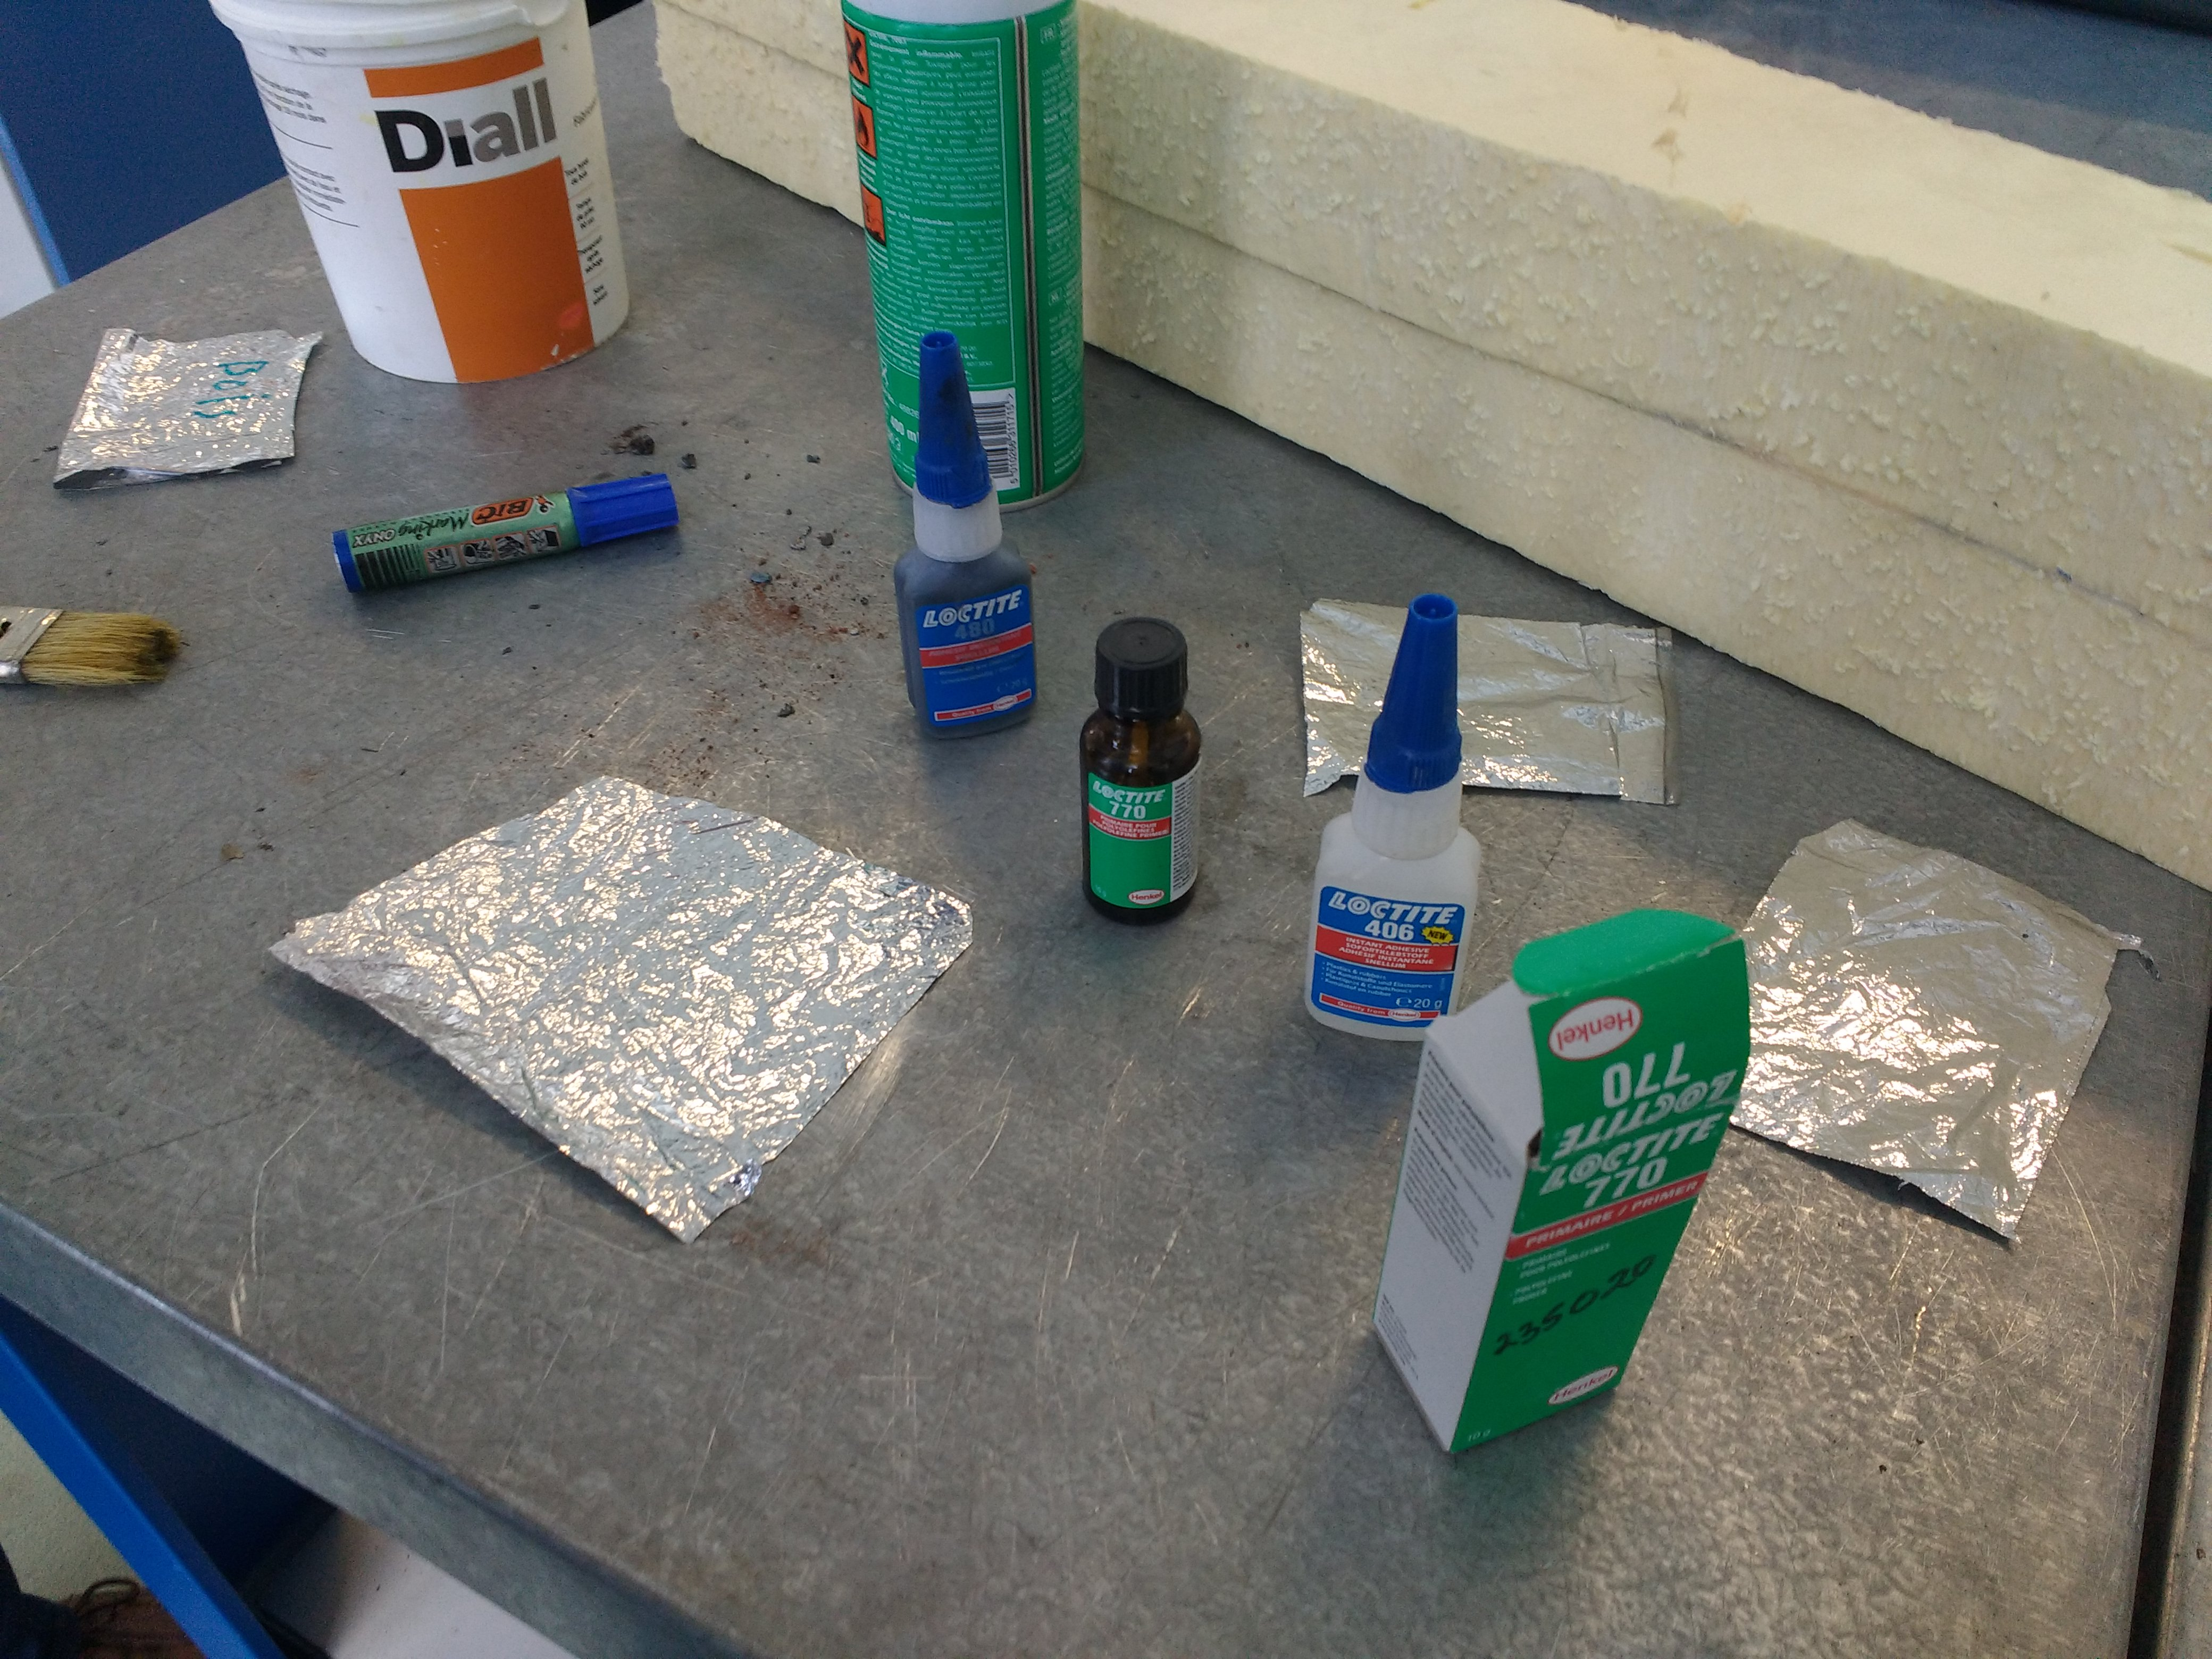
\includegraphics[width=5cm]{../Images/colle2.jpg}
    \end{center}
    \captionof{figure}{A gauche la colle 406 et à droite la colle acétone.}
  \end{multicols}
\end{frame}

\subsection{Modèle}

\begin{frame}
  \begin{center}
    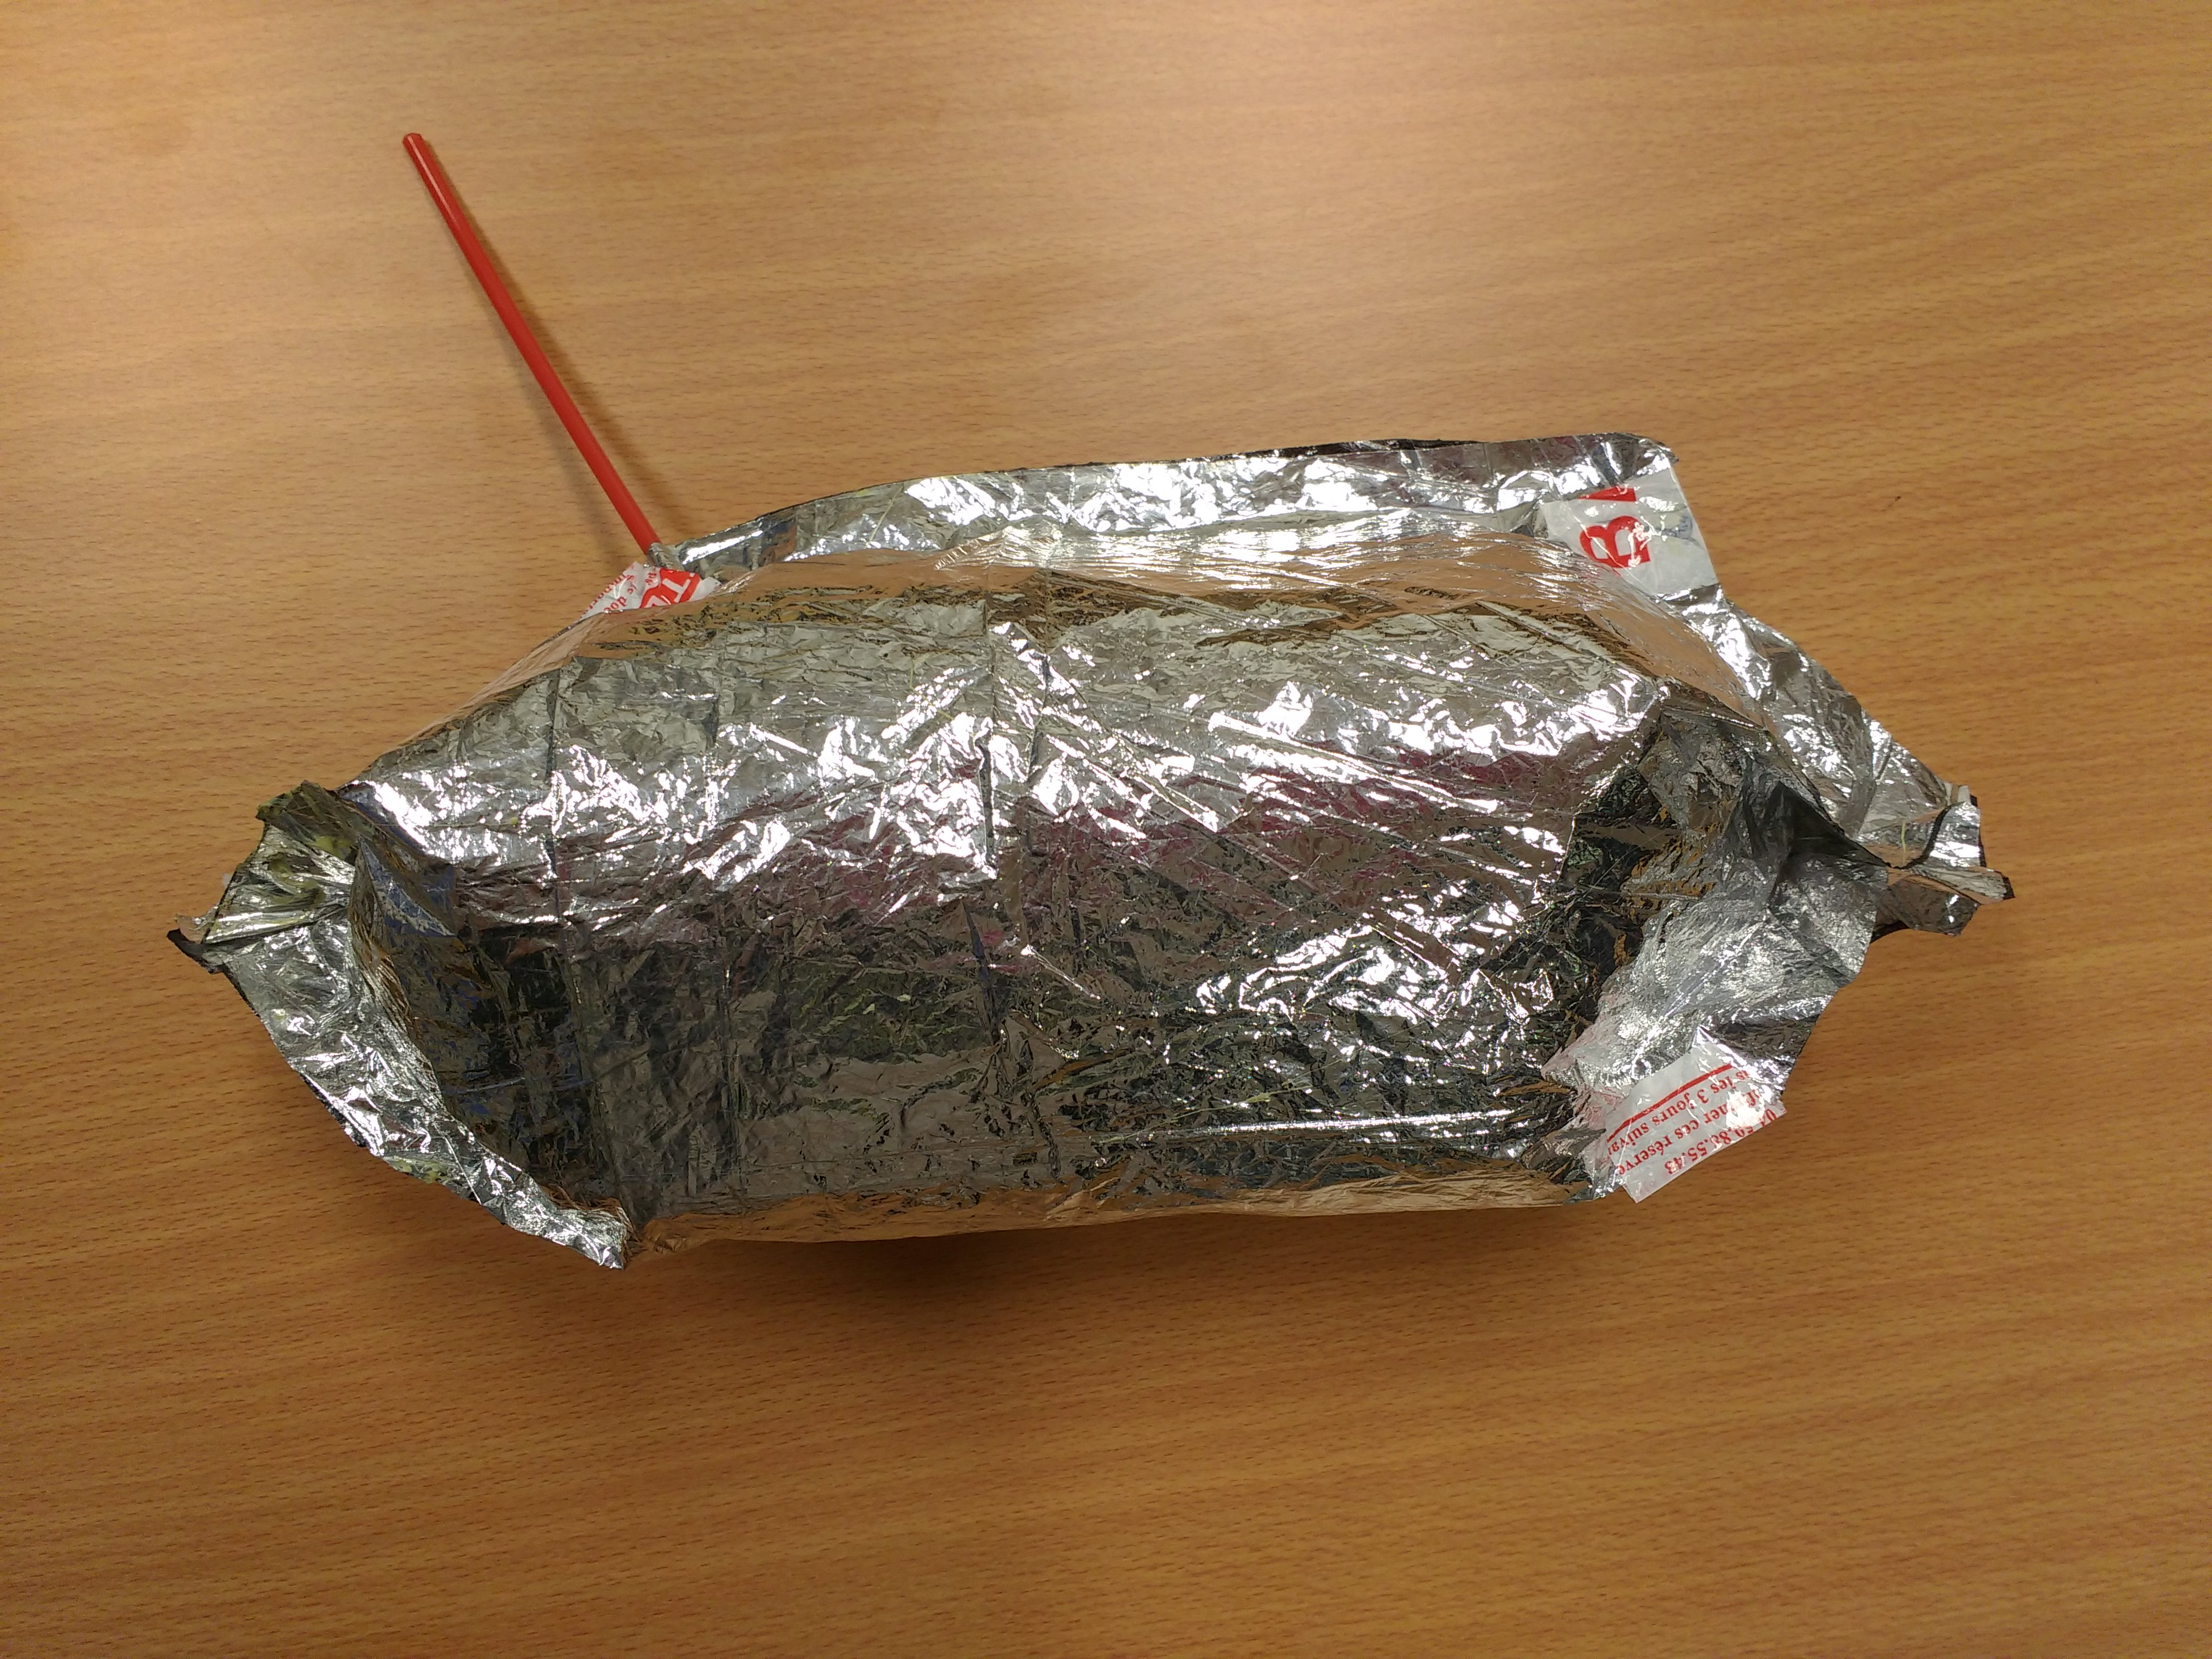
\includegraphics[width=10cm]{../Images/ballon3.jpg}
  \end{center}
\end{frame}

\section{Drone}

\subsection{Modèle}

\begin{frame}
  \begin{multicols}{2}
    Drone XCSOURCE~: \\
    \begin{itemize}
      \item 290 mm diagonale~;
      \item 190 mm longueur~;
      \item 70 mm hauteur~;
      \item moteur EMAX MT2204 2300KV Brushless Motor~;
      \item Accu Lipo Gens Ace 2200Mah 11.1V 25C 3S~;
      \item 450 g.
    \end{itemize}
    \newpage
    \begin{center}
      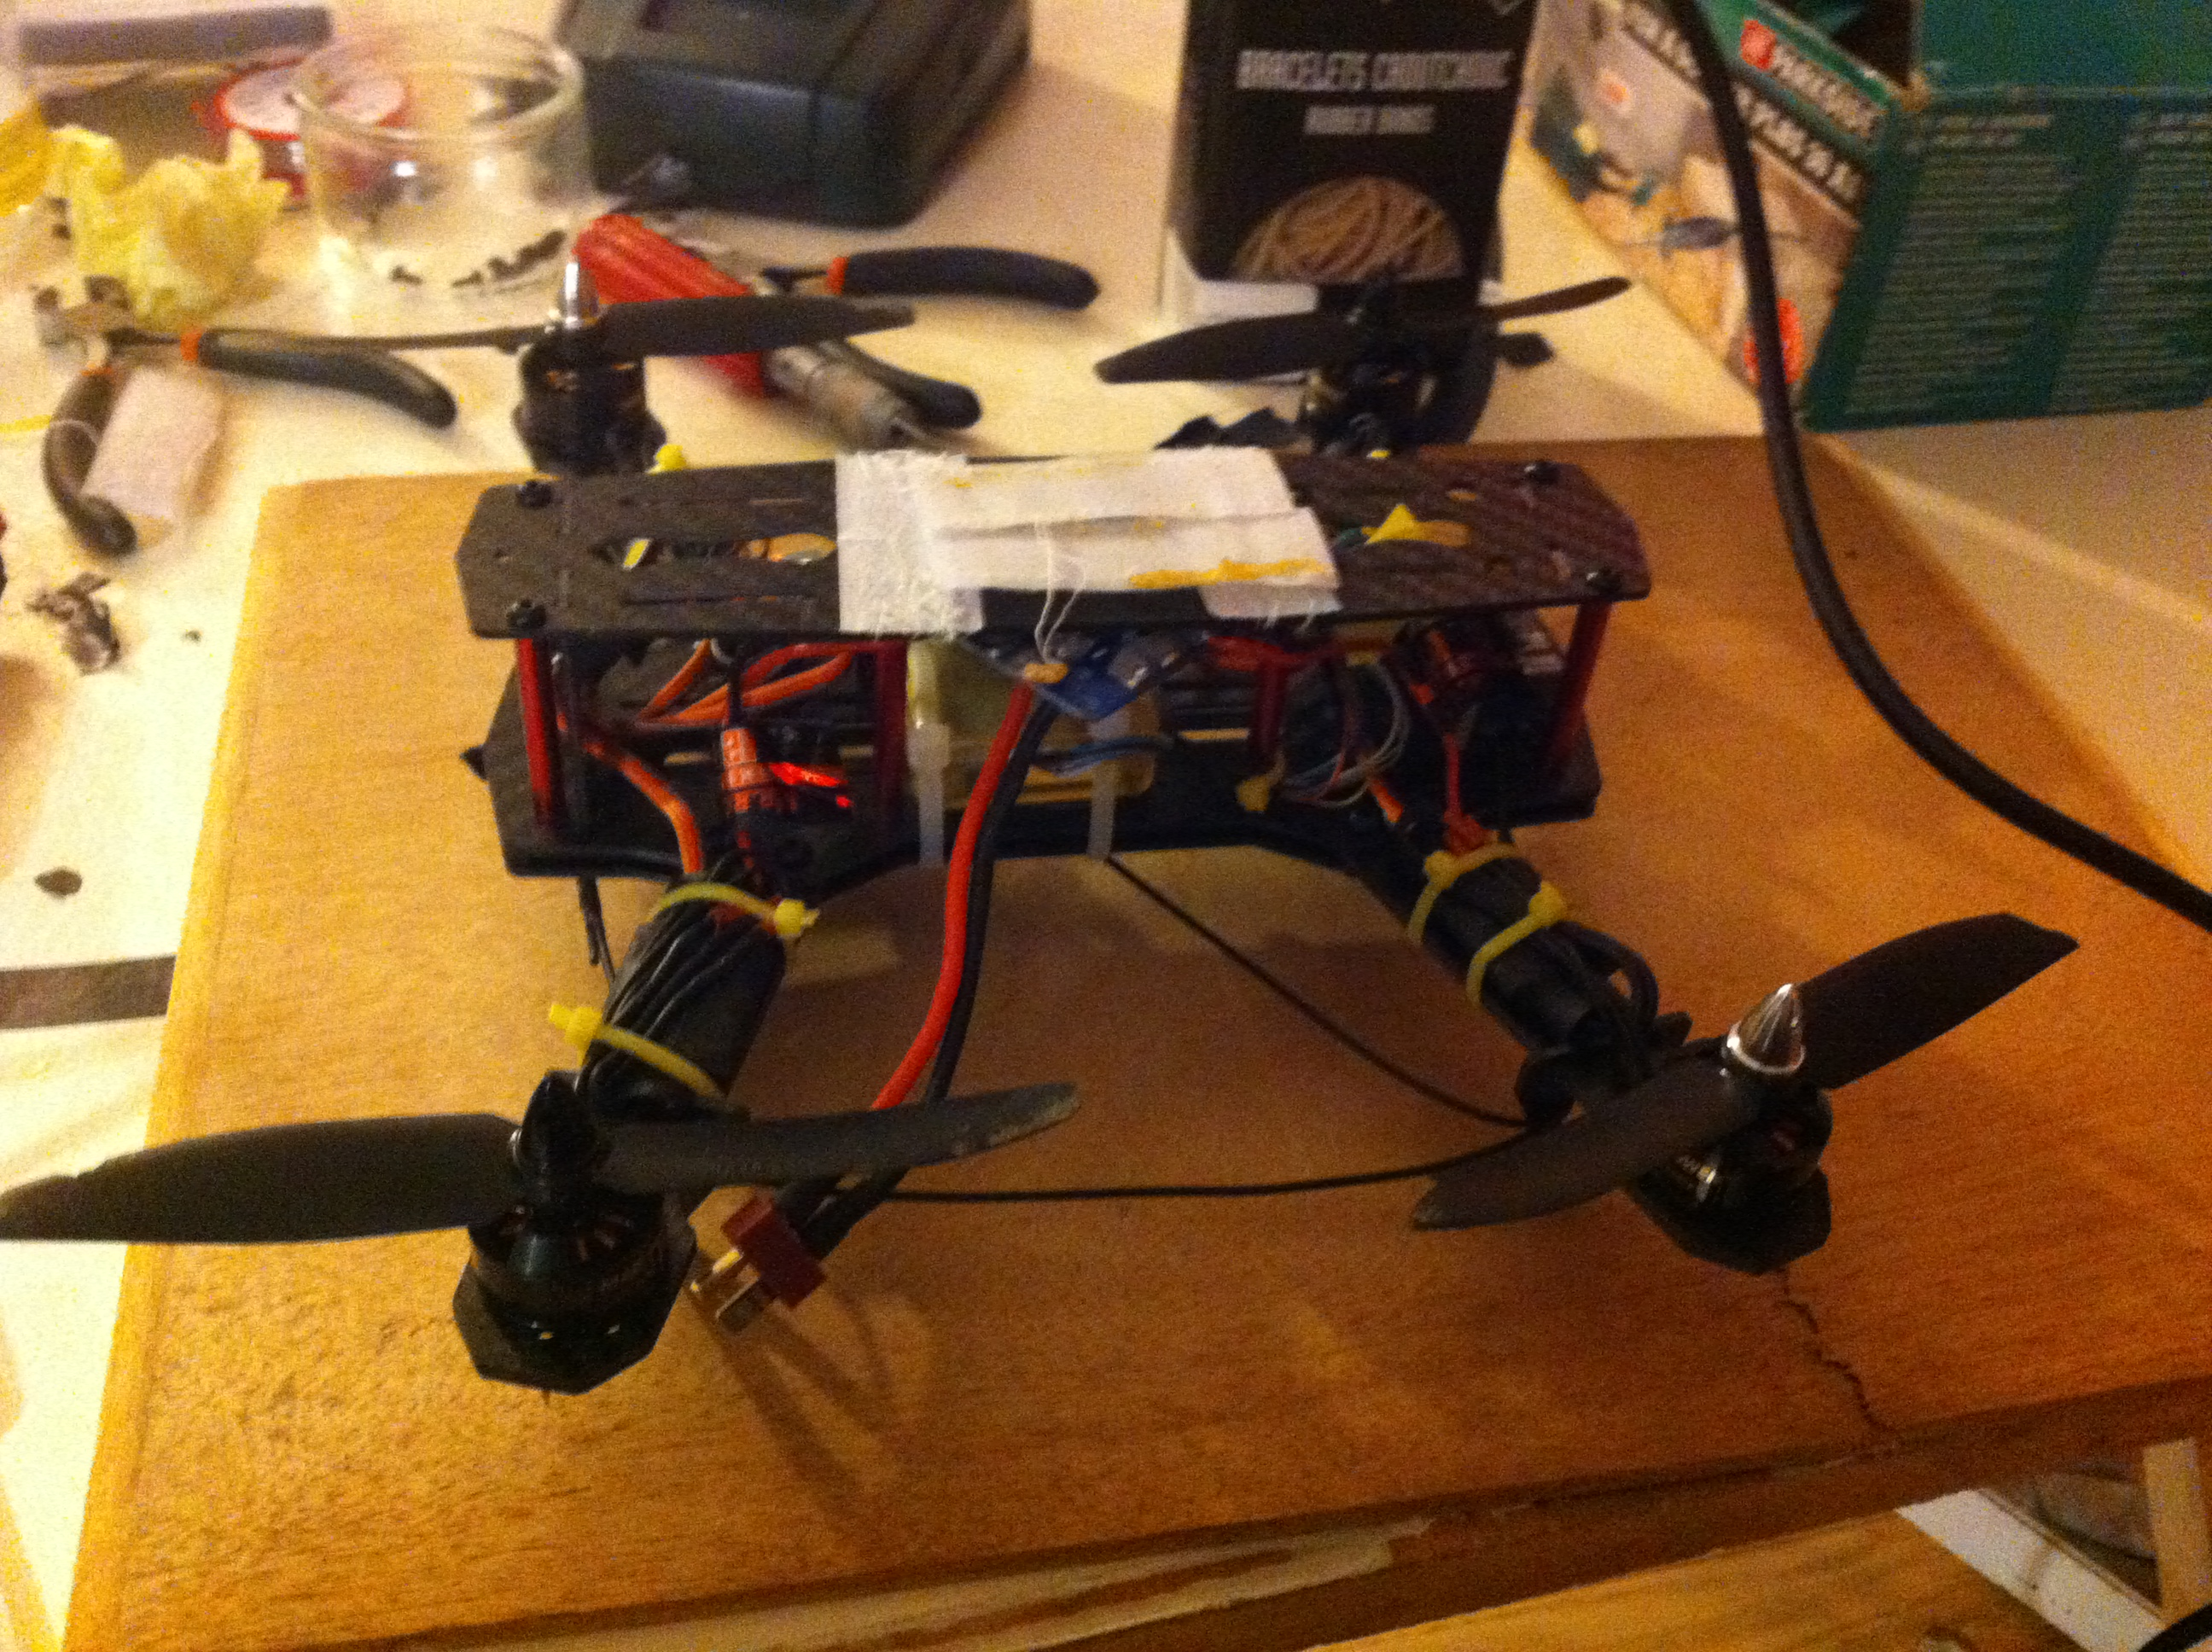
\includegraphics[width=6cm]{../Images/drone.JPG}
    \end{center}
    \captionof{figure}{Drone XCSOURCE.}
  \end{multicols}
\end{frame}

\subsection{Capacité et poids}

\section{Aérodynamisme}

\subsection{Équation de traînée}
\begin{frame}{Équation de traînée}
 But : que le drone soit le moins sensible à l'air possible \\
 Force de traînée matérialisée par l'équation \\
 \begin{center}
  \boxed{\displaystyle{\frac12 \times \rho \times S \times Cx \times V^2}}
 \end{center}
 Avec~:
 \begin{itemize}
  \item $\rho$ la masse volumique du fluide dans lequel a lieu le déplacement en $kg.m^{-3}$~;
  \item S la surface~;
  \item Cx le coefficient de traînée~;
  \item V la vitesse relative du mobile par rapport au fluide en $m.s^{-1}$.
 \end{itemize} 
\end{frame}

\subsection{Calcul de Cx}
\begin{frame}{Nombre de Reynolds}
 \begin{center}
  \boxed{\displaystyle{Re = \frac{VL}{\nu}}}
 \end{center}
 Avec~: \\
 \begin{itemize}
  \item V vitesse du fluide en $m.s^{-1}$~;
  \item L diamètre en m~;
  \item $\nu$ Viscosité cinématique en $m^2.s^{-1}$ ($\nu = 15.6 \times 10^6$ pour l'air).
 \end{itemize} 
\end{frame}

\begin{frame}{Calcul de Cx pour la forme retenue}
 Forme la plus proche : sphère \\
 Dépend du type d'écoulement : le nombre de reynolds \\
 \begin{center}
  $\begin{array}{>{\displaystyle}l>{\displaystyle}l>{\displaystyle}l}
   Re < 1 & Cx = & \frac{24}{Re} \medbreak \\
   1 < Re < 10^3 & Cx = & \frac{18.5}{Re^{0.6}} \medbreak \\
   10^3 < Re < 5.10^5 & Cx = & 0.44
  \end{array}$
 \end{center}
\end{frame}

\section{Taches à faire}
\begin{frame}
  \begin{itemize}
    \item terminer les pièces du ballon~;
    \item assembler la structure~;
    \item assembler les ballons~;
    \item tester et calculer l'aérodynamisme~;
    \item calibrer le drone~;
    \item acheter l'helium.
  \end{itemize}
\end{frame}

\end{document}
